\thispagestyle{diendandayvahoctoannone}
\pagestyle{diendandayvahoctoan}
\everymath{\color{diendantoanhoc}}
\graphicspath{{../diendantoanhoc/pic/}}
\blfootnote{$^1$\color{diendantoanhoc}Trường PT Hermann Gmeiner Vinh, Nghệ An.}
\begingroup
\AddToShipoutPicture*{\put(0,616){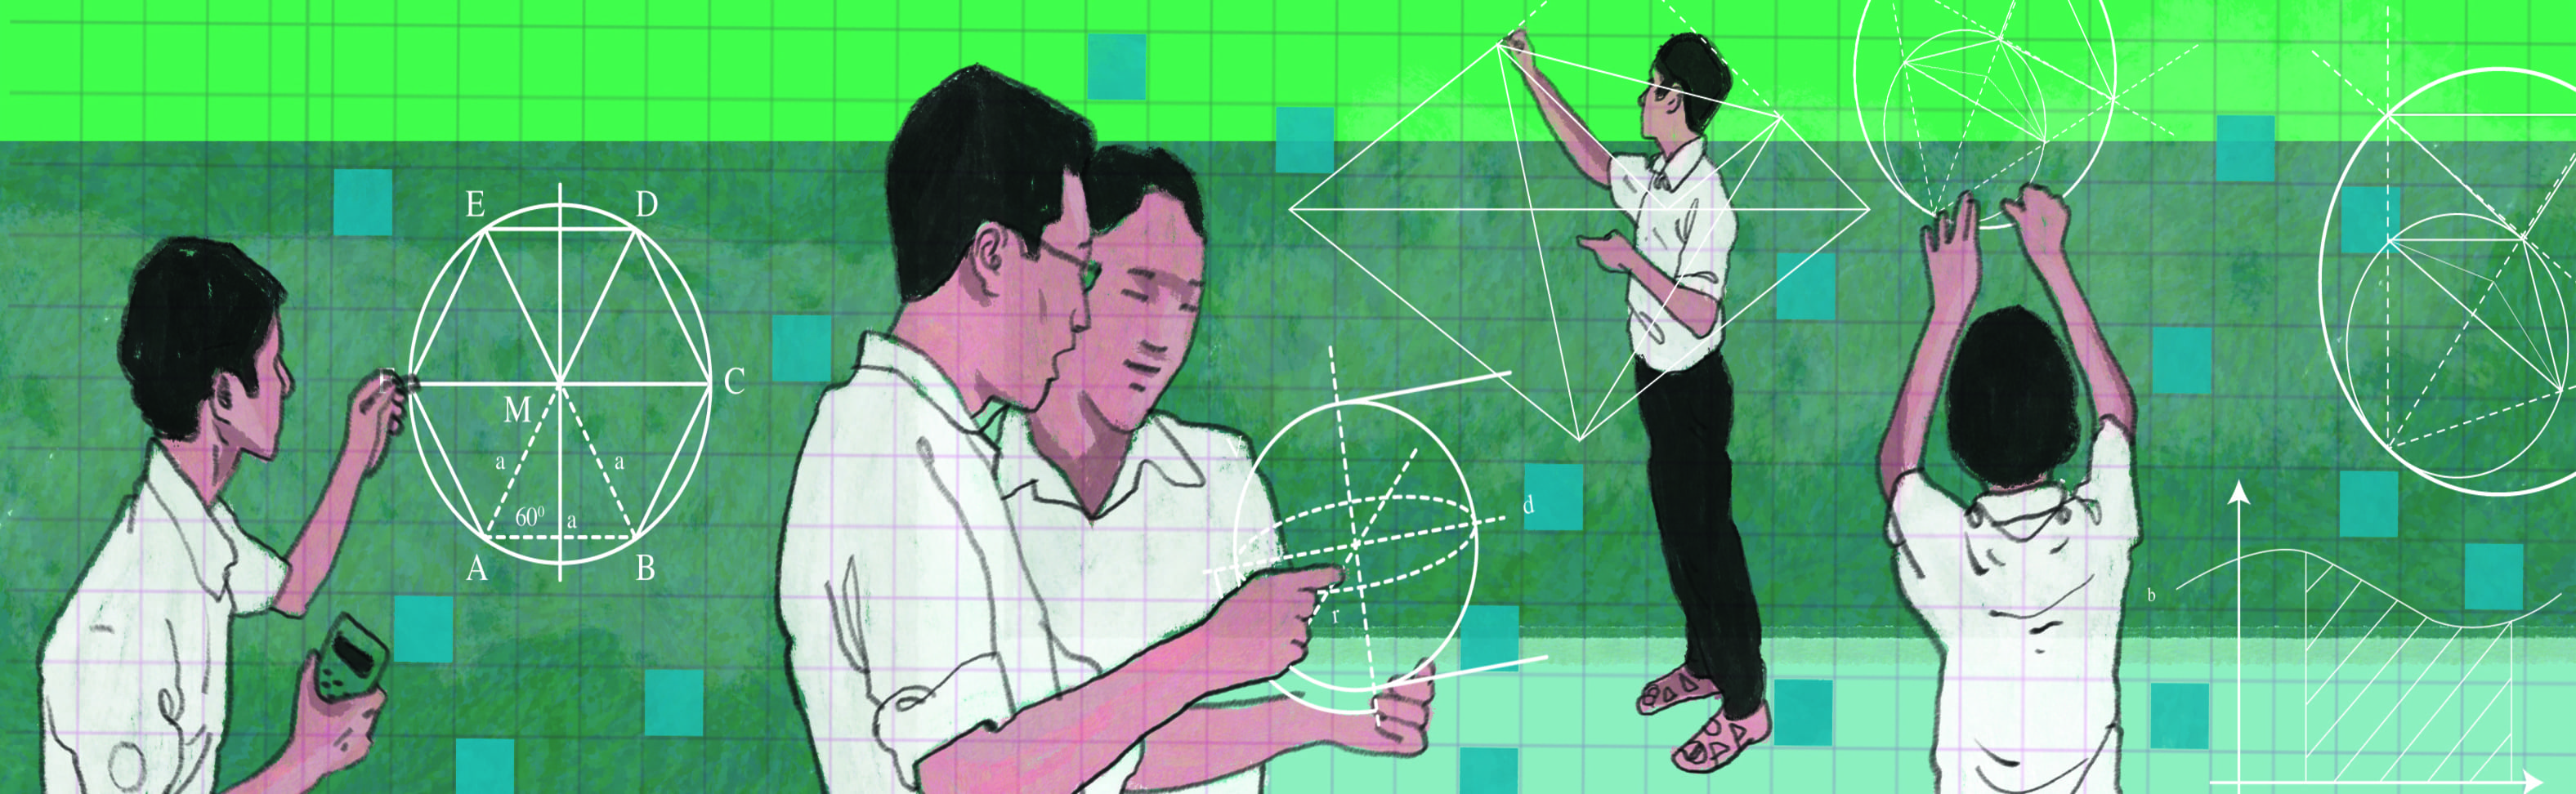
\includegraphics[width=19.3cm]{../bannerdiendan}}}
\AddToShipoutPicture*{\put(110,555){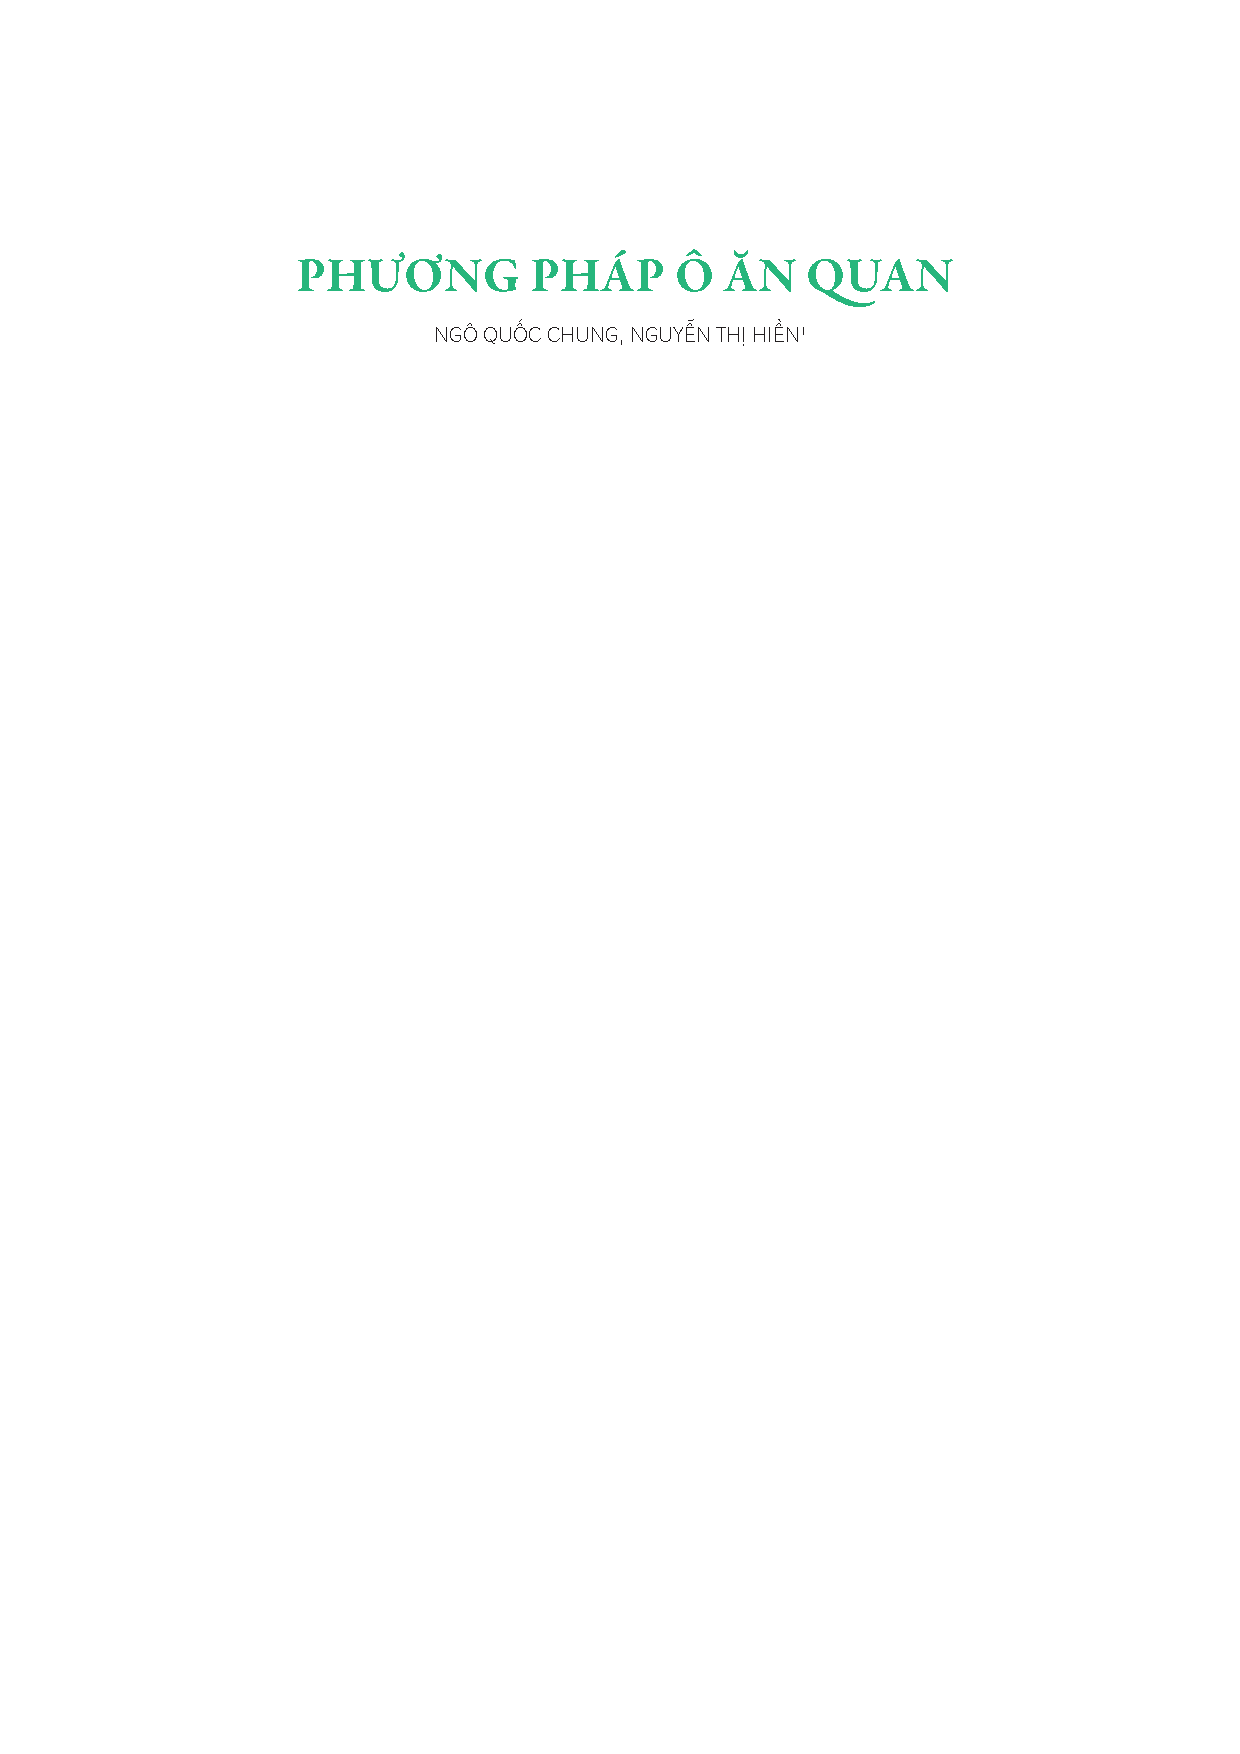
\includegraphics[scale=1]{../tieude1111.pdf}}}  
\centering
\endgroup
\vspace*{160pt} 

\textit{\textbf{\color{diendantoanhoc}LTS.} Trong số này, tạp chí Pi giới thiệu đến bạn đọc một bài viết đạt giải trong kỳ thi Bài giảng và bài viết Toán học, mang tên Hoàng Tuỵ, năm $2022$. Bài viết về chủ đề giảng dạy Toán theo chương trình Toán học $2018$ -- Chương trình Giáo dục Phổ thông mới.}
\begin{multicols}{2}
	\textbf{\color{diendantoanhoc}I.	Đặt vấn đề}
	\vskip 0.1cm
	Trong quá trình tìm các Bài toán thực tế, và xem trò chơi dân gian ``Ô ăn quan" chúng tôi phát hiện ra có sự tương đồng rất lớn giữa bài toán tập hợp hữu hạn với tập hợp các viên sỏi trong trò chơi ``Ô ăn quan". Từ đó chúng tôi nghĩ đến câu hỏi có thể sử dụng phương pháp ô ăn quan để giải các bài Toán tập hợp đếm được, hữu hạn hay không? Áp dụng cho một số Bài toán ban đầu chúng tôi thấy cách giải là rất đẹp và dễ hiểu. Chúng tôi đặt tên cho cách giải đó là ``phương pháp ô ăn quan"
	\vskip 0.1cm
	Với ý muốn là sẽ tạo một cách giải hết sức trực quan chúng tôi quyết định nghiên cứu sâu hơn về các Bài toán tập hợp được phát biểu dưới dạng các bài Toán cổ, ngoài ra chúng ta có thể giải quyết được một số bài ở mức độ phức tạp hơn, khi chứa nhiều biến trong một bài toán.
	\vskip 0.1cm
	Môn toán trong chương trình phổ thông ở cấp Tiểu học giúp học sinh có những kiến thức cơ bản và sơ giản ban đầu về số học, hình học, các yếu tố đại lượng và hình thành các kĩ năng toán học góp phần xây dựng phương pháp học tập, làm việc có kế hoạch, chủ động, sáng tạo giúp các em học tập tốt các môn học khác trong nhà trường và chuẩn bị cho các bậc học tiếp theo. Trong bài viết này, chúng tôi sẽ giải một lớp các Bài toán đó bằng phương pháp ``Ô ăn quan",các ví dụ đưa ra là những bài toán rất quen thuộc ở Tiểu học và cả một số bài tập đề cập ở trên chương trình Toán THPT.
	\vskip 0.1cm
	Với ý tưởng như trên, bài viết sẽ trình bày những kết quả đạt được đạt được trong quá trình chuyển tải phương pháp ``Ô ăn quan" vào giải các bài Toán tập hợp của chương trình Toán Phổ thông mới.
	\vskip 0.1cm
	\textbf{\color{diendantoanhoc}II.	Giải các Bài toán tập hợp bằng phương pháp ``Ô ăn quan"}
	\vskip 0.1cm
	Các bài toán cổ dưới đây thường có nhiều phương pháp giải mà mỗi bậc học có thể được trang bị một cách khác nhau. Tuy nhiên đây là các bài toán có tính logic cao nên học sinh phải có năng lực Toán học khá mới dùng được các phương pháp như vẽ biểu đồ, đặt ẩn giải hệ phương trình, hoặc dùng biểu đồ Venn. Trong phương pháp ô ăn quan, chúng tôi sử dụng những mô tả rất thực tế qua việc dùng những viên sỏi; ô trống và rải sỏi dẫn đến học sinh không cần đòi hỏi quá nhiều kiến thức về Toán vẫn có thể lĩnh hội được.
	\vskip 0.1cm
	\textbf{\color{diendantoanhoc}Bài toán $\pmb{1}$: Gà và chó}
	\begin{center}
		``Vừa gà vừa chó,\\
		Bó lại cho tròn,\\
		$36$ con, $100$ chân chẵn."
	\end{center}
	Hỏi có bao nhiêu con gà, bao nhiêu con chó?
	\vskip 0.1cm
	\textit{Lời giải.}
	Theo bài ta có: tổng số con gà và con chó có tất cả $36$ con và $100$ chân.
	\vskip 0.1cm
	Bây giờ ta vẽ $36$ ô và dùng $100$ viên sỏi. Trong $36$ ô, mỗi ô ta rải vào $2$ viên sỏi hết $72$ viên sỏi, còn lại $28$ viên sỏi. Rải tiếp $28$ viên sỏi còn lại vào các ô, mỗi ô thêm $2$ viên sỏi. Khi đó, có $14$ ô chứa $4$ viên sỏi và $22$ ô chứa $2$ viên sỏi. Vậy ta có $14$ con chó và $22$ con gà.
	\begin{figure}[H]
		\vspace*{-5pt}
		\centering
		\captionsetup{labelformat= empty, justification=centering}
		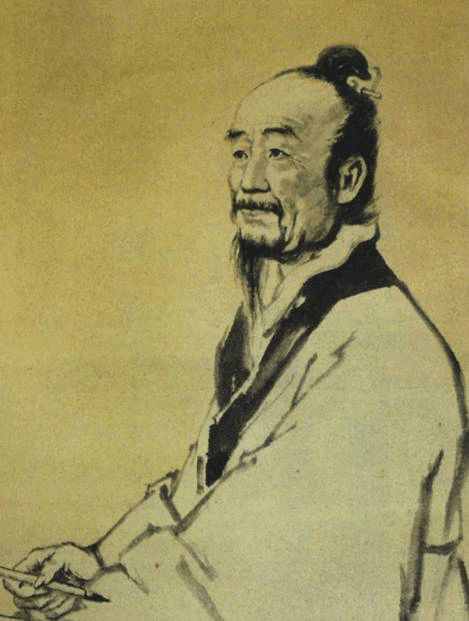
\includegraphics[width= 1\linewidth]{1}
		\vspace*{-15pt}
	\end{figure}
	\textbf{\color{diendantoanhoc}Bài toán $\pmb2$: Thuyền to -- Thuyền nhỏ}
	\begin{center}
		``Thuyền to chở được $6$ người,\\
		Thuyền nhỏ chở được $4$ người là đông.\\
		Một đoàn trai gái sang sông,\\
		$10$ thuyền to nhỏ giữa dòng đang trôi.\\
		Toàn đoàn có cả $100$ người, Trên bờ còn $48$ người đợi sang"
	\end{center}
	Hỏi có bao nhiêu thuyền to, bao nhiêu thuyền nhỏ
	\vskip 0.1cm
	\textit{Lời giải}.
	Toàn đoàn có $100$ người, trên bờ còn $48$ người đợi sang, như vậy có $52$ người đang ngồi trên $10$ thuyền.
	\vskip 0.1cm
	Theo bài ta có: Tổng số thuyền nhỏ và to là $10$ thuyền, $52$ người.
	\vskip 0.1cm
	Bây giờ ta vẽ $10$ ô và dùng $52$ viên sỏi. Trong $10$ ô mỗi ô ta rải vào $4$ viên sỏi hết $40$ viên sỏi, còn lại $12$ viên sỏi. Bỏ tiếp $12$ viên sỏi còn lại vào các ô, mỗi ô thêm $2$ viên. Khi đó, có $6$ ô chứa $6$ viên sỏi và $4$ ô chứa $4$ viên sỏi. Hay có $6$ thuyền to và $4$ thuyền nhỏ.
	\begin{figure}[H]
		\vspace*{5pt}
		\centering
		\captionsetup{labelformat= empty, justification=centering}
		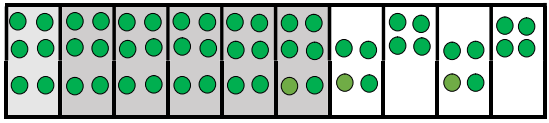
\includegraphics[width= 1\linewidth]{2}
		\vspace*{-15pt}
	\end{figure}
	\textit{Nhận xét.}
	Thông qua những ví dụ trên ta thấy phương pháp ô ăn quan sử dụng những trực quan cụ thể, giúp học sinh dễ dàng thực hiện và ghi nhớ cách làm đồng thời tìm ra kết quả chính xác.
	\vskip 0.1cm
	Ví dụ trên đã yêu cầu học sinh vận dụng được sự mềm dẻo, linh hoạt trong suy nghĩ để giải quyết bài toán. Đó là một yếu tố rất cần thiết, tránh sự cứng nhắc rập khuôn theo những phương pháp đã dẫn đến những cách giải cồng kềnh hoặc bế tắc.
	\vskip 0.1cm
	\textbf{\color{diendantoanhoc}Bài toán $\pmb3$: Bài toán lợn và gà}
	\begin{center}
		Tối qua đếm đàn lợn gà\\
		Thấy được trăm mắt còn đầu năm mươi\\
		Một trăm hai chục chân tròn\\
		Đố bạn biết có bao nhiêu gà và lợn?
	\end{center}
	\textit{Lời giải.}
	Có $50$ cái đầu nên tổng số lợn và gà là $50$ con và tổng số là $120$ chân. Bây giờ ta vẽ $50$ ô tượng trưng cho $50$ con, và lấy $120$ viên sỏi tượng trưng cho $120$ cái chân.
	\vskip 0.1cm
	Bây giờ ta sẽ rải đầy kín tất cả các ô, với mỗi ô hoặc hai viên sỏi, hoặc $4$ viên sỏi. Khi đó số ô có $4$ viên tức là có $4$ chân chính là lợn, số ô có $2$ viên tức là có $2$ chân chính là gà.
	\vskip 0.1cm
	Rõ ràng khi rải đầy các ô có hai viên mỗi ô, thì hết $100$ viên, nên thừa $20$ viên, $20$ viên còn lại rải đủ cho $10$ ô, và do đó để thêm mỗi ô $2$ viên. Vậy số ô có $4$ viên là $10$ nên số lợn là $10$ con, còn lại số ô có $2$ viên là $40$ ô vậy có $40$ gà.
	\begin{figure}[H]
		\vspace*{-5pt}
		\centering
		\captionsetup{labelformat= empty, justification=centering}
		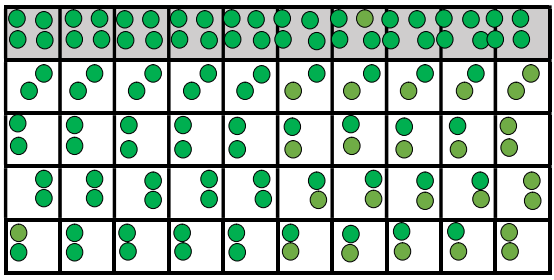
\includegraphics[width= 1\linewidth]{3}
		\vspace*{-15pt}
	\end{figure}
	\textbf{\color{diendantoanhoc}Bài toán $\pmb4$: Bài toán ``Thương nhau cau sáu bổ ba"}
	\begin{center}
		`Thương nhau cau sáu bổ ba\\
		Ghét nhau cau sáu bổ ra làm mười.\\
		Mỗi người một miếng trăm người,\\
		Có mười bảy quả hỏi người ghét yêu"?
	\end{center}
	Hỏi có bao nhiêu quả cau ghét và bao nhiêu quả cau yêu.
	\vskip 0.1cm
	\textit{Lời giải.}
	Ta coi $17$ quả cau là $17$ ô vuông và $100$ miếng cau chia cho $100$ người là $100$ viên sỏi. Trong $17$ ô vuông, mỗi ô vuông rải $3$ viên sỏi hết $51$ viên sỏi, còn lại $49$ viên sỏi. Rải tiếp $49$ viên còn lại vào các ô, mỗi ô thêm $7$ viên. Khi đó, có $7$ ô chứa $10$ viên sỏi và $10$ ô chứa $3$ viên sỏi. Hay có $30$ người tương ứng với $10$ quả cau bổ $3$ và $70$ người ghét ứng với $7$ quả cau bổ $10$.
	\begin{figure}[H]
		\vspace*{-5pt}
		\centering
		\captionsetup{labelformat= empty, justification=centering}
		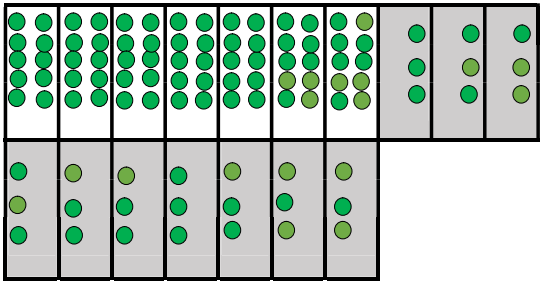
\includegraphics[width= 1\linewidth]{4}
		\vspace*{-15pt}
	\end{figure}
	\textbf{\color{diendantoanhoc}Bài toán $\pmb6$: (Buôn cà phê)}
	\vskip 0.1cm
	Người nọ mua một số cafe tốt và một số cafe xấu trộn lại cân nặng $50$ kg, trả tất cả $7.800\$$. Biết rằng giá $1$ kg cafe tốt $180\$$, giá $1$ kg cafe xấu $120\$$. Hỏi người ấy mua mỗi hạng cafe mấy kg?
	\vskip 0.1cm
	\textit{Lời giải}.
	Ta coi mỗi ô là $1$ kg cà phê, có $50$ kg cà phê nên sẽ có $50$ ô, bây giờ ta sẽ xem mỗi viên sỏi là $60\$$, tổng cộng là $7800\$$ nên sẽ ứng với $130$ viên sỏi. Sau đó ta sẽ rải sỏi vào các ô, mà mỗi ô chỉ nhận $2$ viên $=120\$$ hoặc $3 $viên $=180\$$, số ô có $3$ viên chính là cà phê tốt, số ô chỉ có $2$ viên chính là cà phê xấu. Đầu tiên ta rải đủ $50$ ô, mỗi ô $2$ viên thì còn lại $30$ viên, ta tiểp tục rải $30$ viên còn lại mỗi ô thêm $1$ viên cho đến khi hết sỏi. Ta có hình vẽ sau.
	\begin{figure}[H]
		\vspace*{5pt}
		\centering
		\captionsetup{labelformat= empty, justification=centering}
		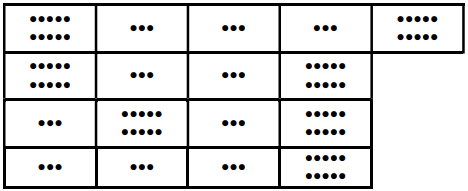
\includegraphics[width= 1\linewidth]{5}
		\vspace*{-15pt}
	\end{figure}
	Nhìn vào bảng ta thấy có $30$ ô chứa $3$ viên sỏi, vậy có $30$ kg cà phê tốt, có $20$ ô chứa hai viên sỏi nên có $20$ kg cà phê xấu.
	\vskip 0.1cm
	Bây giờ ta sẽ giải các bài Toán tập hợp có độ phức tạp cao hơn, đó là những bài toán và có từ $3$ biến trở lên. Những bài toán này nếu giải bằng các cách thông thường sẽ hết sức phức tạp và đòi hỏi rất nhiều kỹ thuật. Nhưng với phương pháp ``Ô ăn quan" ta sẽ có một lời giải rất dễ hiểu, đẹp đẽ và học sinh Tiểu học cũng có thể hiểu được.
	\vskip 0.1cm
	\textbf{\color{diendantoanhoc}Bài toán $\pmb7$:}
	\vskip 0.1cm
	Lớp $5A$ có $35$ học sinh (HS) làm bài kiểm tra toán cuối Kỳ II. Đề bài gồm có $3$ bài toán. Giáo viên chủ nhiệm lớp báo cáo với Nhà trường rằng: Cả lớp mỗi em đều làm được ít nhất một bài, trong đó $20$ em giải được bài toán thứ nhất, $14$ HS giải được bài toán thứ hai, $10$ HS giải được bài toán thứ ba, $5$ HS giải được bài toán thứ hai và thứ ba, $2$ HS giải được bài toán thứ nhất và thứ hai, chỉ có một HS được $10$ điểm vì đã giải được cả ba bài. Học sinh nào giải được bài $3$ thì làm ít nhất thêm được một bài khác.
	Hỏi lớp học đó có bao nhiêu HS không dự kiểm tra?
	\vskip 0.1cm
	\textit{Lời giải}.
	Trước hết ta vẽ bảng gồm có $35$ ô ứng với $35$ em học sinh lớp $5A$. Ta lấy $20$ tấm thẻ ký hiệu là số $B1$ ứng với số lần giải được bài toán $1$, lấy $14$ thẻ ký hiệu là $B2$ ứng với $14$ lần giải được bài toán $2$, $10$ tấm thẻ đánh dấu là $B3$ ứng với $10$ lượt giải được bài toán $3$. Bây giờ ta sẽ rải thẻ vào các ô theo quy tắc đã cho. Đầu tiên ta rải $20$ tấm thẻ $B1$ vào $20$ ô, sau đó ta rải đến tấm thẻ $B2$ vào $2$ ô có thẻ $B1$ và thêm $12$ ô trống, hết thẻ $B2$ bây giờ ta rải thẻ $B3$, $1$ tấm thẻ vào ô đã có $2$ thẻ $B1$ và $B2$, tiếp tục rải $5$ thẻ vào các ô chỉ có thẻ $B2$, do làm được bài $3$ thì sẽ làm được hơn một bài do đó sẽ rải $4$ thẻ còn lại vào các ô chỉ có $B1$. Sau khi rải hết thẻ mà ô nào còn trống có nghĩa là học sinh đó không đi thi.
	\begin{figure}[H]
		\vspace*{-5pt}
		\centering
		\captionsetup{labelformat= empty, justification=centering}
		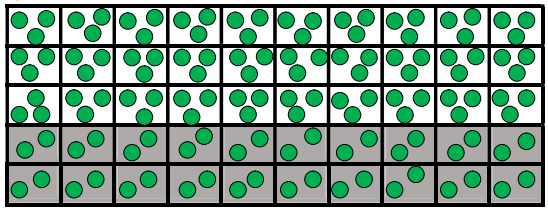
\includegraphics[width= 1\linewidth]{6}
		\vspace*{-15pt}
	\end{figure}	
	Nhìn vào bảng sau khi rải hết các thẻ theo quy tắc trên ta thấy còn lại chỉ có $3$ ô trống nên có $3$ em học sinh không tham gia thi cuối kỳ II.
	\begin{figure}[H]
		\vspace*{-5pt}
		\centering
		\captionsetup{labelformat= empty, justification=centering}
		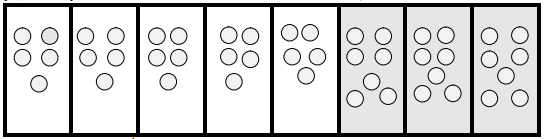
\includegraphics[width= 1\linewidth]{7}
		\vspace*{-15pt}
	\end{figure}
	\textbf{\color{diendantoanhoc}Bài toán $\pmb8$:} 
	\vskip 0.1cm
	Trong một hội nghị có $100$ đại biểu tham dự, mỗi đại biểu nói được một hoặc hai trong ba thứ tiếng: Nga, Anh hoặc Pháp. Có $39$ đại biểu chỉ nói được tiếng Anh, $35$ đại biểu nói được tiếng Pháp, có $12$ đại biểu biết $2$ thứ tiếng trong đó $8$ đại biểu nói được cả tiếng Anh và tiếng Nga. Hỏi có bao nhiêu đại biểu chỉ nói được tiếng Nga, bao nhiêu đại biểu chỉ nói được tiếng Pháp?
	\vskip 0.1cm
	\textit{Lời giải}.
	\begin{figure}[H]
		\vspace*{-5pt}
		\centering
		\captionsetup{labelformat= empty, justification=centering}
		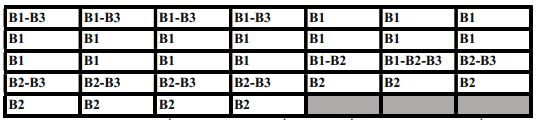
\includegraphics[width= 1\linewidth]{8}
		\vspace*{-15pt}
	\end{figure}
	Ta vẽ $100$ ô tương ứng với $100$ đại biểu. Ta sẽ làm $39$ thẻ chữ $A$ ứng với $35$ người nói được tiếng Anh, $35$ thẻ chữ $P$ ứng với $35$ người biết nói tiếng Pháp và $8$ thẻ chữ $NA$ ứng với số lượng biết nói tiếng Nga, gọi thẻ chữ $N$ là ký hiệu biết nói tiếng Nga.
	\vskip 0.1cm
	Đầu tiên, ta sẽ rải $39$ thẻ $A$ vào $39$ ô. Ta rải tiếp $35$ thẻ chữ $P$ vào các ô trống tiếp theo, tiếp tục rải tiếp $8$ thẻ $NA$ vào các ô trống còn lại. Bây giờ ta sẽ rải thẻ chữ $N$, vì mỗi đại biểu nói được ít nhất một thứ tiếng, nên những ô trống còn lại ta sẽ rải chữ $N$ vào. Do có $12$ đại biểu biết nói hai thứ tiếng mà lại có $8$ người nói Anh và Nga do đó chắc chắn có $4$ người nói tiếng Pháp thì nói được tiếng Nga (vì không thể cùng biết cả Anh và Pháp) do đó ta sẽ rải $4$ thẻ chữ $N$ vào $4$ ô có chữ $P$. Khi đó ô nào mà chỉ có một mình chữ N là chỉ nói được tiếng Nga, những ô chỉ có chữ $P$ là chỉ nói được tiếng Pháp. Nhìn vào bảng ta thấy: có $18$ ô chữ $N$ vậy có $18$ đại biểu chỉ nói được tiếng Nga. Có $31$ ô chỉ có chữ $P$ nên có $31$ đại biểu chỉ nói được tiếng Pháp
	\vskip 0.1cm
	\textbf{\color{diendantoanhoc}Bài toán $\pmb9$.}
	\vskip 0.1cm
	$50$ bạn học sinh lớp $12A$ đều đội $1$ trong hai loại mũ: Mũ cứng hoặc mũ mềm, đi $1$ trong $2$ loại giày đen hoặc nâu, mặc $1$ trong $2$ loại áo: trắng hoặc xanh. Có $18$ bạn đội mũ mềm, $19$ bạn đi giầy đen, $11$ bạn có áo trắng. Hỏi có thể chắc chắn có ít nhất bao nhiêu bạn vừa đi giày nâu, vừa đội mũ cứng và mặc áo xanh?
	\vskip 0.1cm
	\textit{Lời giải}.
	Ta sẽ vẽ bảng gồm $50$ ô, ta kí hiệu thẻ chữ $M$, $C$ lần lượt ứng với đội mũ mềm và mũ cứng, thẻ $Đ$, $N$ lần lượt cho giày đen và giày nâu, thẻ $T$, $X$ cho mặc áo trắng và áo xanh.
	\begin{figure}[H]
		\vspace*{-5pt}
		\centering
		\captionsetup{labelformat= empty, justification=centering}
		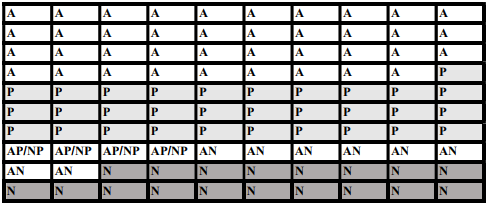
\includegraphics[width= 1\linewidth]{9}
		\vspace*{-15pt}
	\end{figure}
	Vì có $18$ bạn đội mũ mềm ta rải $18$ thẻ $M$ vào $18$ ô, các ô trống còn lại ta rải chữ $C$ cho các bạn đội mũ cứng, ta rải tiếp $19$ thẻ $D$ vào hết các bạn có thẻ chữ $C$, hết chữ $C$ ta sẽ rải sang chữ $M$, nhiều ô chữ $C$ nhất có thể. Sau đó ta rải $11$ thẻ chữ $T$ vào ô chữ $CN$, hết các ô đó ta sẽ rải sang các ô còn lại, khi hết $11$ thẻ chữ $T$ ta tiếp tục rải chữ $X$ vào tất cả các ô không chứa chữ $T$. Khi đó ô nào mà chữa $3$ chữ $CNX$ thì đó chính là học sinh đi giày Nâu, đội mũ Cứng và mặc áo Xanh.
	\vskip 0.1cm
	Nhìn vào bảng ta thấy chỉ có hai ô có $3$ chữ $CNX$ nên có ít nhất $2$ học sinh đội mũ cứng, đi giày nâu và mặc áo xanh.
	\vskip 0.1cm
	\textit{Nhận xét:} Đây là bài Toán logic khá hóc búa vì nó chứa đến $6$ yếu tố để tác động lên một học sinh, nếu dùng phương pháp suy luận thông thường chúng ta sẽ vấp phải các lý luận khá phức tạp và dễ bị nhầm lẫn. Phương pháp ``Ô ăn quan" cho ta một lời giải rất đẹp đẽ và khá ngắn gọn.
	\vskip 0.1cm
	\textbf{\color{diendantoanhoc}IV. Bài tập đề xuất}
	\vskip 0.1cm
	\textbf{\color{diendantoanhoc}Bài $\pmb1$:} Trong một Hội nghị có $100$ người tham dự, trong đó có $10$ người không biết tiếng Nga và tiếng Anh, có $75$ người biết tiếng Nga và $83$ người biết Tiếng Anh. Hỏi trong hội nghị có bao nhiêu người biết cả $2$ thứ tiếng Nga và Anh?
	\vskip 0.1cm
	\textbf{\color{diendantoanhoc}Bài $\pmb2$:} Một lớp học có $16$ học sinh học giỏi môn Toán; $12$ học sinh học giỏi môn Văn; $8$ học sinh vừa học giỏi môn Toán và Văn; $19$ học sinh không học giỏi cả hai môn Toán và Văn. Hỏi lớp học có bao nhiêu học sinh?
	\vskip 0.1cm
	\textbf{\color{diendantoanhoc}Bài $\pmb3$:} Một lớp có $45$ học sinh. Mỗi em đều đăng ký chơi ít nhất một trong hai môn: bóng đá và bóng chuyền. Có $35$ em đăng ký môn bóng đá, $15$ em đăng ký môn bóng chuyền. Hỏi có bao nhiêu em đăng ký chơi cả $2$ môn?
	\vskip 0.1cm
	\textbf{\color{diendantoanhoc}Bài $\pmb4$:} Lớp $12A$ có $20$ học sinh thích bóng đá, $17$ học sinh thích bơi, $36$ học sinh thích bóng chuyền, $14$ học sinh thích bơi và bóng đá, $13$ học sinh thích bơi và bóng chuyền, $15$ học sinh thích bóng đá và bóng chuyền, $10$ học sinh thích cả $3$, $12$ học sinh không thích môn nào cả . Tính số học sinh của lớp $12A$?
	\vskip 0.1cm
	\textbf{\color{diendantoanhoc}Bài $\pmb5$:} Lớp $10A$ có $40$ học sinh trong đó có $10$ bạn học sinh giỏi Toán, $15$ bạn học sinh giỏi Lý, và $22$ bạn không giỏi môn học nào trong hai môn Toán, Lý. Hỏi lớp 10A có bao nhiêu bạn học sinh vừa giỏi Toán vừa giỏi Lý?
	\vskip 0.1cm
	\textbf{\color{diendantoanhoc}Bài $\pmb6$:} (Thi giữa kỳ $1$ -- Trường PTTH Lý Nhân Tông, Hà Nội) Lớp $10A$ có $45$ học sinh trong đó có $15$ học sinh thích chơi đá bóng, $12$ học sinh thích chơi bóng rổ, $6$ học sinh thích chơi cả $2$ môn. Số học sinh không thích chơi cả $2$ môn thể thao trên là:
	\vskip 0.1cm
	\textbf{\color{diendantoanhoc}Bài $\pmb7$:} Lớp $10A$ có $7$ học sinh giỏi Toán, $5$ học sinh giỏi Lý, $6$ học sinh giỏi Hóa, $3$ học sinh giỏi cả Toán và Lý, $4$ học sinh giỏi cả Toán và Hóa, $2$ học sinh giỏi cả Lý và Hóa, $1$ học sinh giỏi cả $3$ môn Toán, Lý, Hóa. Số học sinh giỏi đúng hai môn học của lớp 10A là bao nhiêu.
	\vskip 0.1cm
	\textbf{\color{diendantoanhoc}Tài liệu tham khảo}
	\vskip 0.1cm
	[$1$]	L. V. An, N. T. Sơn, N. T. Thiêm, N. T. H. Anh, N. Q. Chung ($2023$), Nhìn bài toán cổ theo quan điểm Tổ hợp, Kỷ yếu HTKH cấp Trường: ``Nâng cao chất lượng đào tạo ngành Sư phạm trong bối cảnh hiện nay", Trường Đại học Hà Tĩnh, (Hà Tĩnh, ngày $24/3/2023$), $179 - 186$.
	\vskip 0.1cm
	[$2$] Naum Yakolevich Vilenkin -- Dịch giả: Nguyễn Tiến Dũng, Trần Thanh Nam, Nguyễn Chí Thức, Hồ Thị Thảo Trang, \textit{Toán học qua các câu chuyện về Tập hợp}, Tủ sách SPUTNIK, NXB Thế giới, năm $2017$.
	\vskip 0.1cm
	[$3$] Trịnh Hồng Long, \textit{$670$ bài toán đố}, NXB Sống Mới, năm $1970$.
	\vskip 0.1cm
	[$4$] Người dịch: Trần Lưu Cường, Trần Lưu Thịnh, \textit{Những bài toán cổ}, NXB giáo dục, năm $1995$.
	\vskip 0.1cm
	[$4$] Trần Nam Dũng (Tổng chủ biên), Trần Đức Huyên (Chủ biên), Nguyễn Thành Anh -- Vũ Như Thư Hương -- Ngô Hoàng Long -- Phạm Hoàng Quân -- Phạm Thị Thu Thủy, \textit{Sách chân trời sáng tạo -- Toán $10$ -- Tập $1$}, NXB giáo dục Việt Nam, năm $2022$.
	\vskip 0.1cm
	[$5$]	Đỗ Đức Thái (Tổng chủ biên), Phạm Xuân Chung, Nguyễn Sơn Hà, Nguyễn Thị Phương Loan, Phạm Sỹ Nam, Phạm Minh Phương, Phạm Hoàng Quân, \textit{Sách Cánh diều -- Toán $10$ -- Tập $1$}, NXB Giáo dục, năm $2021$	
\end{multicols}